\subsection{Constante}

Assim como as constantes globais utilizadas na linguagem de programação
\acs{PHP} através da função \textit{define}, esta tecnologia também dispõem de
uma maneira que permite definirmos uma constante em uma classe ou em uma 
interface. Da mesma maneira que as propriedades estáticas as constantes podem 
ser acessadas diretamente de dentro do escopo da classe utilizando-se de um 
operador especial denominado \textit{self}, ou ainda, no caso da constante, ser
acessada de fora do escopo da classe através do nome da classe \cite{programmingPhp}.

Quando uma constante de uma classe é definida - da mesma maneira que uma
constante global -  seu valor não poderá ser alterado no decorrer da vida útil
da aplicação. Uma prática comumente utilizada pelos desenvolvedores de software
é definir o nome de uma constante com caixa alta, isto permite que ela seja
identificada rapidamente em um trecho de código. Por conseguinte, uma constante
é um identificador que recebe apenas um valor de inicialização, por conta disto,
seu valor não poderá ser alterado durante a execução do aplicativo.

A seguir na Figura \ref{fig:constante}, é apresentado um exemplo de implementação
de uma constante utilizando a linguagem de programação \acs{PHP}:

\begin{figure}[h!tb]
	\caption{Constante declarada na linguagem PHP}
	\label{fig:constante}

	\centering
	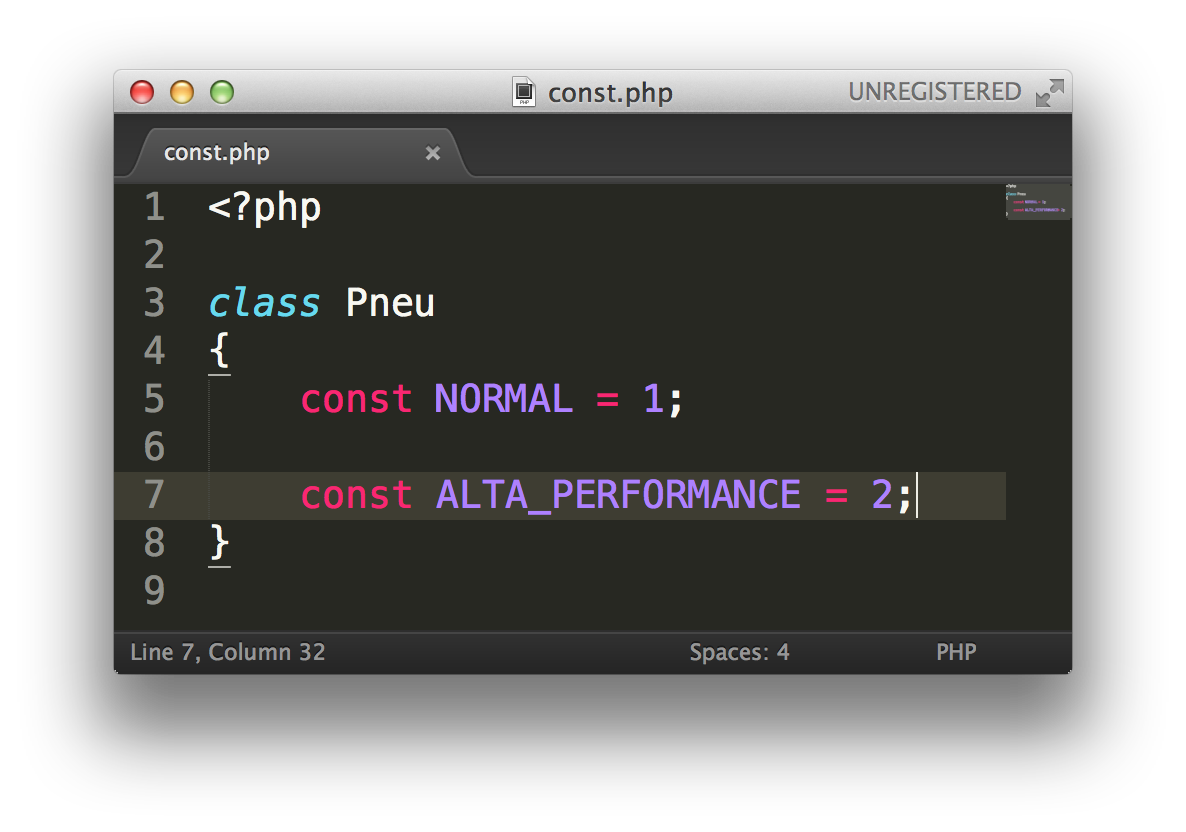
\includegraphics[width=0.75\textwidth]{images/const.png}

	\centering
	\footnotesize Fonte: \fonteOAutor
\end{figure}

\FloatBarrier 	% Este comando impede que as imagens
				% flutuem a partir deste ponto no seu documento

Logo abaixo, é apresentado em detalhes as linhas de código exibidas na Figura 
\ref{fig:constante}:

\begin{enumerate}[a)]
    \item linha 1: vê-se o início da execução de um bloco de código PHP;
    \item linha 3: identifica-se a declaração da classe \textit{Pneu};
    \item linha 5: define-se a constante que representa um pneu normal,
    atribuindo a ela o valor numérico 1, que pode ser um código de
    identificação;
    \item linha 7: informa-se outra constante relativa a outro tipo de pneu,
    neste caso, o de alta performance.
\end{enumerate}

Logo a seguir, será apresentado o conceito de mensagem que permite que os
objetos se comuniquem entre si.
